\subsection{Statistics}
\begin{frame}{Statistics}

\begin{itemize}
\item <1-> Current implementation
	\begin{itemize}
	\item<2-> Primitive
	\item<3-> Based on unsound data
	\end{itemize}
\end{itemize}

\begin{figure}[htbp]
	\begin{center}
	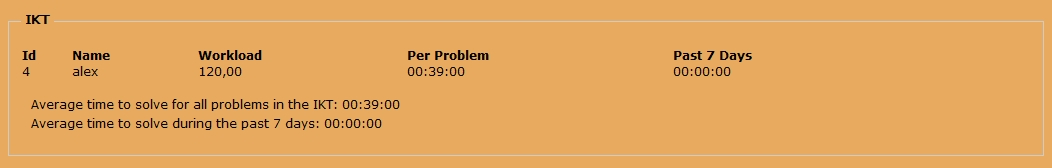
\includegraphics[width=280pt]{input/statistics.jpg}
	%\caption{default}
	%\label{default}
	\end{center}
\end{figure}

\end{frame}

\begin{frame}{Statistics}

\begin{itemize}
\item<1-> Potential improvements
	\begin{itemize}
	\item<2-> Better data:
		\begin{itemize}
		\item<3-> Time solving problems
		\item<4-> Type of problem
		\end{itemize}
	\item<5-> More factors:
		\begin{itemize}
		\item<6-> ``difficulty'' of the submitter
		\item<7-> Working hours of staff
		\end{itemize}
	\item<8-> Better UI
		\begin{itemize}
		\item<9-> Graphical presentation of data
		\item<10-> Show the average time on tags
		\end{itemize}
	\end{itemize}
\end{itemize}

\end{frame}